\documentclass[mathserif, serif, 11pt]{beamer}

\usepackage{amsmath}
\usepackage{amsfonts}
\usepackage{amssymb}
\usepackage[utf8]{inputenc}
\usepackage[T2A]{fontenc}
\usepackage[english, russian]{babel}
\usepackage{graphicx}
\usepackage{ragged2e}
\DeclareGraphicsExtensions{.eps, .png, .jpg, .gif}
\newtheorem{Th}{Теорема}
\usetheme{Madrid}
\usecolortheme{wolverine}

\title[Матрицы]{Матрицы}
\author[Фамилия]{Кузьмин М. Д.}
\institute[МГУ]
{
	Естественно-научный факультет МГУ им.~М.\,В.~Ломоносова
}
\date[Февраль 2024]
{
	Математика\\
	26 февраля 2024
}

\begin{document}
	
	\frame{\titlepage}
	
	\begin{frame}{Определение матрицы}
		\begin{columns}
			\begin{column}{6cm}
				Матрица - это прямоугольная таблица чисел, расположенных по строкам и столбцам. Количество строк и столбцов определяет размер матрицы.
			\end{column}
			\begin{column}{6cm}
				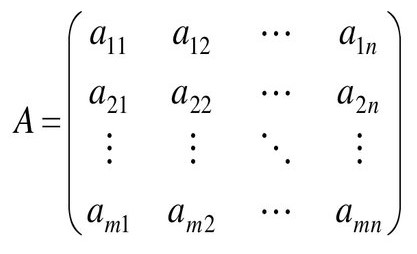
\includegraphics[width=6cm]{matrix.jpg}
			\end{column}
		\end{columns}
	\end{frame}
	
	\begin{frame}{Операции с матрицами}
		\begin{columns}
			\begin{column}{6cm}
				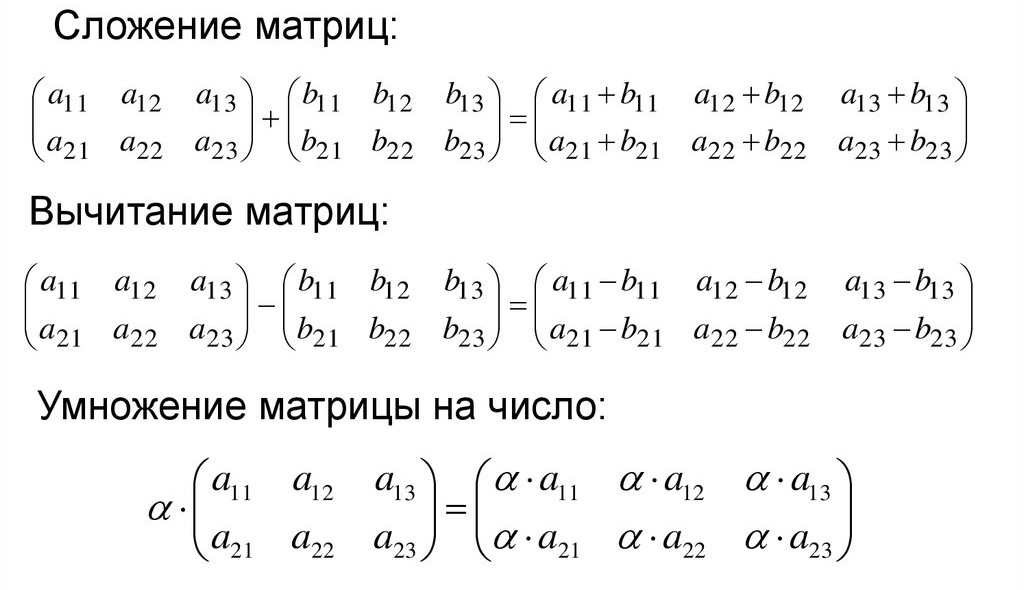
\includegraphics[width=7cm]{oper.jpg}
			\end{column}
			\begin{column}{1cm}
			\end{column}
			\begin{column}{4cm}
				С матрицами можно выполнять различные операции, такие как сложение, вычитание, умножение и транспонирование.
			\end{column}
		\end{columns}
	\end{frame}
	
	\begin{frame}
		\begin{block}{Теорема о сложении матриц}
			Сложение матриц производится поэлементно. То есть, элементы матриц складываются со своими соответствующими элементами в другой матрице.
		\end{block}
		
		\begin{columns}
			\begin{column}{5cm}
				\begin{block}{Пример сложения матриц}
					Пусть есть две матрицы A и B. Тогда их сумма A + B будет матрицей, каждый элемент которой равен сумме соответствующих элементов матриц A и B.
				\end{block}
			\end{column}
			\begin{column}{5cm}
				\begin{block}{Пример умножения матриц}
					Умножение матриц более сложное. Для умножения матрицы A на матрицу B, число столбцов в A должно быть равно числу строк в B.
				\end{block}
			\end{column}
		\end{columns}
	\end{frame}
	
	
	\begin{frame}[fragile]{Реализация матриц в Python}
		\begin{verbatim}
			import numpy as np
			
			A = np.array([[1, 2], [3, 4]])
			B = np.array([[5, 6], [7, 8]])
			
			print("A + B = ")
			print(A + B)
			
			print("A * B = ")
			print(np.dot(A, B))
		\end{verbatim}
	\end{frame}
	
	\begin{frame}
		\begin{center}
			\LARGE
			Спасибо за внимание!
		\end{center}
	\end{frame}
\end{document}